\documentclass[11pt,a4paper]{article}
\usepackage[utf8]{inputenc}
\usepackage[T1]{fontenc}
\usepackage[margin=2.5cm]{geometry}
\usepackage{amsmath}
\usepackage{array}
\usepackage{booktabs}
\usepackage{enumitem}
\usepackage{tikz}
\usetikzlibrary{positioning}
\usepackage{graphicx}
\graphicspath{{figures/}}
\usepackage[hidelinks]{hyperref}

\usepackage{xurl}
\makeatletter\g@addto@macro\UrlBreaks{\do\_}\makeatother
\newcommand{\code}[1]{\path{#1}}
\newcommand{\doi}[1]{\href{https://doi.org/#1}{doi:#1}}
\newcommand{\ra}{\raggedright\arraybackslash}
\sloppy

\title{Indirect retinotopy:\\why spatial order in a map does not show a coordinate update}
\author{Francesco Mannella}
\date{October 4, 2026 \\ \small branch \code{saliencies}; working note, not yet a paper section}

\begin{document}
\maketitle

\begin{abstract}
\noindent
Accounts of visual stability across voluntary saccades read the spatial order
found in cortical maps (retinotopic receptive fields, predictive remapping, gain
fields) as evidence that a coordinate system is held and updated. We argue that
\emph{retinotopy can be indirect, inherited from retinal input and from alignment
with the motor map, so observing it does not show that a coordinate system is
updated}. A map organised by the global differences among retina-centred images
keeps position as one locally ordered dimension, and an observer who maps it with
spots will call it retinotopic; sensory maps aligned with a retinal-vector motor
map inherit its order as well. A black-box probe of the project's maps, which are
trained only on global differences among foveal images, finds significant
retinotopy in all of them (z between 20 and 57 in 40 maps of 20 runs of the champion
configuration), and in 32 of 40 the order exceeds what prototype-space topography
alone gives. If so, stability can be carried by the
neighbourhood relation between a saccade's address and its effect on a shared
lattice, with no global frame and no predictive model of space. We set out the
argument, what the project's model does and does not show, the limits of the
evidence, and the predictions that would separate the view from remapping and
spatiotopy.
\end{abstract}

\section{The question and the standard answers}

Each voluntary saccade moves every image feature to a new retinal position, yet
the scene appears stable. The companion review
(\code{docs/visual_stability_review.tex}) organises the literature into two lines
and a deflationary alternative.

\begin{itemize}[nosep]
  \item \textbf{Spatiotopic.} Eye position scales retinotopic responses (gain
    fields), giving head- or world-centred coding in a minority of neurons in
    VIP, MST and V6A, and spatiotopic effects in human psychophysics and imaging
    (Burr and Morrone, 2011; Fabius et al., 2019).
  \item \textbf{Retinotopic remapping.} A corollary discharge (CD) shifts
    receptive fields or attention pointers to the post-saccadic location before
    the eye lands (Duhamel et al., 1992; Sommer and Wurtz, 2006; Cavanagh et al.,
    2010; Rolfs et al., 2011).
  \item \textbf{Deflationary.} Little is carried; the world is assumed stable
    and sampled again, and vision is the mastery of sensorimotor contingencies
    (Bridgeman et al., 1975; O'Regan and No\"e, 2001).
\end{itemize}

\section{The inference under test}

The three answers differ on what is updated, but they share an inference: spatial
order observed in a map is taken as evidence that the area holds a coordinate
system, and that something updates it at each saccade. Remapping needs a signal
stating where each stimulus will land, which is a model of how the retinal image
changes under the saccade. Spatiotopic coding needs a global frame and an
eye-position signal, and post-saccadic eye-position signals in parietal cortex are
slow and unreliable (Xu et al., 2012; Morris et al., 2012). The sensorimotor account
asks the system to master the relation between every movement and the change it
causes, which is again general predictive knowledge.

This note examines the inference, not the data. The findings stand; the question
is what they entitle us to conclude about the organisation of the maps in which
they are observed.

\section{Indirect retinotopy}
\label{sec:indirect}

A map can show retinotopic order without being retinotopic in the sense the
inference needs. There are two routes.

\paragraph{Route 1: inherited from the input.} The training data of any visual map
are retina-centred: objects occupy positions on the retina, so position is one
dimension of the data. A self-organising map with a neighbourhood constraint
organises itself around the dominant differences among its inputs, and keeps
position as one embedded dimension, smoothly represented even when other
dimensions dominate. Probing such a map with localised stimuli then reveals
spatial order. This is a geometric by-product of topographic learning on
spatially structured input, not a dedicated map of space
(\code{knowledgebase/remapping_alternative/visual_remapping_caveat.tex}).

\paragraph{Route 2: inherited from alignment.} The saccade is itself a retinal
vector. If the sensory maps are aligned with a motor map whose units are tuned to
saccade vectors, as sensory maps are with collicular motor maps, neighbouring
sensory units come to prompt similar saccades. The sensory map then shows order in
retinal displacement without having been organised around position.

\paragraph{Retinotopic-proper versus indirect.} Both routes are compatible with
what an observer sees when mapping receptive fields. What distinguishes the two
readings is the role of position in the map (Table~\ref{tab:criteria}). The
distinction is a gradient. It is strongest where input is pooled and
feature-dominated (higher parietal and frontal areas) and weakest in V1, where
positional variance dominates natural input.

\begin{table}[h]
\centering\footnotesize
\setlength{\tabcolsep}{3pt}
\begin{tabular}{@{}>{\ra}p{3.1cm}>{\ra}p{5.8cm}>{\ra}p{5.8cm}@{}}
\toprule
Property & Retinotopic-proper & Indirect \\
\midrule
Organising axis & Position in the visual field & Content (shape, view, action); position is one dimension \\
Global structure & Smooth map of the field & Local order; global order set by content \\
Receptive-field centres & Span the field & Not usable as a criterion with soft readout, which compresses the range (Section~\ref{sec:probe}) \\
Readout & Order visible with any readout & Weak with hard winner-take-all, clear with population readout \\
Role in stability & Supports a coordinate update & No coordinate needed; neighbourhood relations \\
Training statistics & Little effect on layout & Layout changes with the content statistics \\
\bottomrule
\end{tabular}
\caption{Operational criteria. Measures: variance explained by position against
content, dependence on readout, dependence on training statistics.}
\label{tab:criteria}
\end{table}

\section{How the retinotopy test works}
\label{sec:test}

This section explains the test used in the SOM note and in Section~\ref{sec:probe}.
It is a \emph{black-box} test: it asks only what the map does when a small stimulus
is shown at a known position, as an electrophysiologist would, without using the
training data, the loss or the labels. The question is: do units that are neighbours
on the map respond to nearby positions?

\paragraph{Relation to standard retinotopic mapping.} This is not the field's
standard method, and it should not be called that. In fMRI, retinotopy is mapped
with phase-encoded stimuli, a rotating wedge and an expanding ring, which give each
voxel a preferred polar angle and eccentricity from the phase of its response; area
borders come from the visual field sign (Engel et al., 1994; Sereno et al., 1995;
DeYoe et al., 1996; Engel et al., 1997). Population receptive field (pRF) modelling
fits a Gaussian receptive field to each voxel (Dumoulin and Wandell, 2008; Wandell
and Winawer, 2015). In electrophysiology, receptive fields are mapped with spots
and bars (Hubel and Wiesel, 1962). All of these estimate each unit's preferred
position directly and judge the map by its smoothness, its field sign or its
confluences. The SOM literature has its own measures of neighbourhood preservation,
the topographic product (Bauer and Pawelzik, 1992), the topographic function
(Villmann et al., 1997) and the topographic error (Kiviluoto, 1996), but they are
computed in input or prototype space, not on the positions of probe stimuli. Table~\ref{tab:standard} says, measure by measure, what corresponds to what.

\begin{table}[h]
\centering\footnotesize
\setlength{\tabcolsep}{3pt}
\begin{tabular}{@{}>{\ra}p{3.0cm}>{\ra}p{4.9cm}>{\ra}p{1.9cm}>{\ra}p{4.6cm}@{}}
\toprule
Part of the measure & Counterpart in the field's methods & Relation & Difference \\
\midrule
1. Spot at a known position
  & Localised stimulus: spots and bars in electrophysiology (Hubel and Wiesel, 1962);
    wedge, ring and bar sweeps in fMRI and pRF mapping
  & Same in kind
  & Spots are static and at random positions; mapping sweeps a stimulus through the field
    so that response timing carries the position \\
2. Soft readout, hard readout
  & Population response (voxel or population signal) and best single unit
  & Analogous
  & Readout is a modelling choice here, not a measurement property \\
3. RF centre $c_j$
  & Preferred position of a unit or voxel: from the response phase (phase-encoded
    mapping) or the fitted pRF centre (Dumoulin and Wandell, 2008)
  & Closest match
  & A response-weighted mean of the spot positions (a centre of mass), not a phase
    or a fitted Gaussian \\
4. $\rho$
  & Relation between cortical distance and visual-field distance, which underlies
    cortical magnification and the smooth progression of polar angle and eccentricity
    across cortex
  & Related in concept
  & Rank-based and global over all pairs of units; it has no sign, so it cannot
    detect mirror reversals, which the visual field sign (Sereno et al., 1995) does \\
5. $z$
  & Statistical thresholding in mapping, for example on the reliability of a voxel's
    response to the stimulus
  & Different object
  & The field's thresholds test that a unit responds; $z$ tests that the map is ordered \\
6--7. Shuffled-layout control, gain, $p$
  & None found
  & Ours
  & Addresses a confound specific to topographic maps: neighbouring prototypes are
    similar, so responses are smooth whatever the stimulus \\
RF range
  & Visual-field coverage of RF centres; pRF size
  & Related in concept
  & Soft readout compresses the centres, so the range is not comparable with pRF size \\
Participation ratio
  & None found
  & Ours
  & Counts responding units per spot \\
\bottomrule
\end{tabular}
\caption{Correspondence between the spot-probe measure and the field's retinotopic
mapping methods. ``None found'' means none in the references checked. The exact
statistic used for thresholding differs among the papers listed and was not checked
in each.}
\label{tab:standard}
\end{table}

In short: steps 1 and 3 (a localised stimulus and an RF centre per unit) are what the
test shares with standard practice, and the RF centres can be compared with phase- or
pRF-derived positions. Step 4 is related in concept to cortical magnification, but is
a different statistic. Steps 5 to 7 and the participation ratio are not standard.
``Retinotopy found'' below therefore means found by this spot-probe protocol. A
stronger version would also run phase-encoded or pRF-style mapping on the maps
(Section~\ref{sec:probe}, open items).

\paragraph{The object tested: a self-organising map (SOM).} A SOM is a grid of units,
here $10\times10$. Each unit $j$ has a position $p_j$ on the grid (its row and
column) and a prototype $w_j$, a template of the same size as an input image
($16\times16\times3=768$ numbers). For an input image $x$ the winner is the unit
whose prototype is closest, $\arg\min_j\|x-w_j\|^2$. Training moves the winner and its
grid neighbours towards the input, so units that are close on the grid end up with
similar prototypes. This is \emph{topography in prototype space}: nearby units hold
similar templates. Nothing in training refers to where in the image anything is; each
image is compared as a whole. The project's maps are trained the same way, with the
anchor term of Section~\ref{sec:stability}.

\begin{figure}[h]
\centering
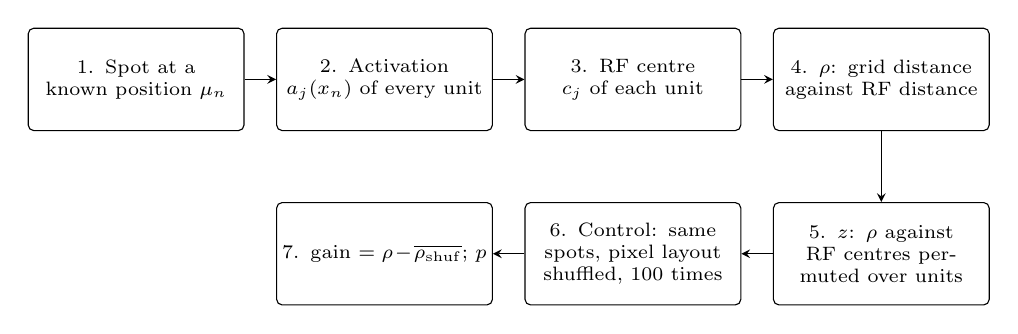
\begin{tikzpicture}[>=stealth,
  b/.style={draw,rounded corners=2pt,align=center,font=\scriptsize,minimum height=1.3cm,text width=2.6cm,inner sep=2pt}]
\node[b] (a) {1. Spot at a known position $\mu_n$};
\node[b,right=0.4cm of a] (b) {2. Activation $a_j(x_n)$ of every unit};
\node[b,right=0.4cm of b] (c) {3. RF centre $c_j$ of each unit};
\node[b,right=0.4cm of c] (d) {4. $\rho$: grid distance against RF distance};
\node[b,below=0.9cm of d] (e) {5. $z$: $\rho$ against RF centres permuted over units};
\node[b,left=0.4cm of e] (f) {6. Control: same spots, pixel layout shuffled, 100 times};
\node[b,left=0.4cm of f] (g) {7. gain $=\rho-\overline{\rho_{\mathrm{shuf}}}$; $p$};
\draw[->] (a)--(b); \draw[->] (b)--(c); \draw[->] (c)--(d); \draw[->] (d)--(e);
\draw[->] (e)--(f); \draw[->] (f)--(g);
\end{tikzpicture}
\caption{The black-box test, step by step. Steps 1--5 follow the SOM note's protocol;
steps 6--7 are the control added here.}
\label{fig:pipeline}
\end{figure}

\paragraph{Step 1: spots.} Present $N$ images that each contain one Gaussian bump
\begin{equation}
  I_n(x,y)=\exp\!\Bigl(-\tfrac{(x-\mu_{x,n})^2+(y-\mu_{y,n})^2}{2\sigma^2}\Bigr),
\end{equation}
centred at a known position $\mu_n=(\mu_{x,n},\mu_{y,n})$ and of width $\sigma$
(3 pixels here), the same on all three colour channels. A spot is a marker, like a
flashed dot in physiology; it does not look like the training images.

\paragraph{Step 2: activations.} Two ways of reading the map's response.
\emph{Hard} (winner-take-all): only the winner is active, $a_j=1$ for the winning
unit and 0 for the others. \emph{Soft} (population): every unit responds, with
\begin{equation}
  a_j(x)=\frac{\exp(-\|x-w_j\|^2/\tau^2)}{\sum_k\exp(-\|x-w_k\|^2/\tau^2)},\qquad
  \tau^2=2\,\mathrm{median}_n\bigl(\min_j\|x_n-w_j\|^2\bigr),
\end{equation}
so closer prototypes respond more, and $\tau$ is set from the data so that the
response is neither a single winner nor flat. Soft readout is the analogue of
population activity, hard readout of the best single unit.

\paragraph{Step 3: receptive-field (RF) centre.} For each unit, the RF centre is the
average spot position weighted by how strongly the unit responded,
\begin{equation}
  c_j=\frac{\sum_n a_j(x_n)\,\mu_n}{\sum_n a_j(x_n)} .
\end{equation}
It is the place the unit ``looks at''. A unit that never responds has no RF centre.

\paragraph{Step 4: the correlation $\rho$.} For every pair of units $(j,k)$ take the
grid distance $d^{\mathrm{grid}}_{jk}=\|p_j-p_k\|$ and the RF distance
$d^{\mathrm{RF}}_{jk}=\|c_j-c_k\|$. Then
\begin{equation}
  \rho=\mathrm{Spearman}\bigl(\{d^{\mathrm{grid}}_{jk}\},\{d^{\mathrm{RF}}_{jk}\}\bigr),
\end{equation}
the rank correlation over all pairs. $\rho=1$ means that the further apart two units
are on the grid, the further apart the places they look at; $\rho=0$ means no
relation; $\rho<0$ means neighbours look at distant places. A toy case: three units
at grid positions 0, 1 and 3 have grid distances 1, 2, 3 for the pairs (0,1), (1,3),
(0,3); if their RF centres are at 2, 5 and 11 pixels the RF distances are 3, 6, 9,
the two orders agree, and $\rho=1$. A map that is retinotopic by design gives a high
$\rho$; $\rho$ is the \emph{size} of the order.

\paragraph{Step 5: the score $z$.} To ask how surprising $\rho$ is, shuffle which
unit owns which RF centre, recompute $\rho$ (here 100 times), and express the
observed value in standard deviations above those shuffled values,
\begin{equation}
  z=\frac{\rho-\overline{\rho_{\mathrm{perm}}}}{\mathrm{sd}(\rho_{\mathrm{perm}})} .
\end{equation}
By convention $z>3$ counts as significant. $z$ measures \emph{significance}, not
size: with 100 units there are 4950 pairs, so even a modest $\rho$ gives a large $z$.
Both are reported.

\paragraph{Step 6: the control, and why it is needed.} Neighbouring units have
similar prototypes (topography), so they respond similarly to \emph{any} input,
spots included. Their RF centres can therefore come out similar, and $\rho$ positive,
because the prototypes are smooth, not because the prototypes carry spatial
information. The control separates the two. Shuffle the pixel positions of every
spot with one fixed random permutation (the same for all spots), which keeps the
amplitude and the content statistics but destroys the spatial arrangement, and keep
the original labels $\mu_n$. Probe again and compute $\rho_{\mathrm{shuf}}$; repeat
with 100 different permutations. Then
\begin{equation}
  \mathrm{gain}=\rho-\overline{\rho_{\mathrm{shuf}}},\qquad
  p=\frac{1+\#\{\rho_{\mathrm{shuf}}\ge\rho\}}{1+100}.
\end{equation}
The gain is the part of $\rho$ that depends on the spatial arrangement of the
spot; $p$ is the chance of getting $\rho$ from shuffled layouts alone. The smallest
possible $p$ is $1/101\approx0.01$.

\paragraph{Two further quantities.} \emph{RF range}: for each axis the spread of the
RF centres, $(\max_j c_j-\min_j c_j)/(\text{side}-1)$, averaged over the two axes; it
is the fraction of the fovea they cover. \emph{Participation ratio} (PR): the
number of units that respond to a spot, $(\sum_j a_j)^2/\sum_j a_j^2$, averaged over
spots; it is 1 for hard readout.

\begin{table}[h]
\centering\footnotesize
\setlength{\tabcolsep}{3pt}
\begin{tabular}{@{}>{\ra}p{1.6cm}>{\ra}p{3.7cm}>{\ra}p{3.0cm}>{\ra}p{6.1cm}@{}}
\toprule
Symbol & Name & Range & Reading \\
\midrule
$\rho$ & Rank correlation of grid distance and RF distance & $-1$ to $1$ & Size of the order. 1: perfectly ordered; 0: none \\
$z$ & Score against permuted RF centres & Unbounded & Significance of $\rho$. Above 3: significant. Grows with the number of pairs \\
gain & $\rho$ minus mean $\rho_{\mathrm{shuf}}$ & About $-1$ to $1$ & Order that depends on the spatial arrangement of the spot; near 0: none beyond topography \\
$p$ & Share of shuffled layouts with $\rho_{\mathrm{shuf}}\ge\rho$ & 0.01 to 1 & Chance of $\rho$ from shuffled layouts; below 0.05: spatial \\
RF range & Spread of RF centres & 0 to 1 & Fraction of the fovea covered by the centres \\
PR & Participation ratio & 1 to 100 & Units responding per spot \\
\bottomrule
\end{tabular}
\caption{Glossary of the statistics used in the probe.}
\label{tab:glossary}
\end{table}

\paragraph{How to read the outcomes.}
\begin{itemize}[nosep]
  \item \textbf{$z$ high, gain high ($p<0.05$).} The RF centres are ordered on the
    grid and the order depends on the spatial arrangement of the spot: retinotopic
    order is found beyond topography. Expected for a map retinotopic by design.
  \item \textbf{$z$ high, gain near 0 ($p>0.05$).} The spot-probe test says
    ``retinotopic'', but shuffled layouts do as well: the order is prototype
    topography.
  \item \textbf{$z$ high, gain moderate, $p<0.05$.} Real spatial order beyond
    topography, weaker than by design.
\end{itemize}

\section{Evidence and its limits}

\begin{itemize}[nosep]
  \item \textbf{Maps are a general format, including frontoparietal cortex.}
    Topographic maps with confluent foveae are found in human frontal and
    parietal cortex and carry attention, working-memory and saccade signals
    (Silver and Kastner, 2009; Mackey et al., 2017); retinotopy extends into areas
    not primarily spatial (Arcaro and Livingstone, 2017), with five visual-field maps
    along the intraparietal sulcus (Swisher et al., 2007).
  \item \textbf{A SOM trained on shape keeps local spatial order.} The SOM note
    applied the test of Section~\ref{sec:test} to a $10\times10$ self-organising map
    trained on 20{,}919 images of coloured rectangles varying in shape, size,
    orientation, aspect, colour and position, using 20{,}400 Gaussian spots
    (\code{knowledgebase/remapping_alternative/detecting_topographic_organization.pdf}).
    With hard readout $\rho\approx0.18$ (weak); with soft readout
    $\rho\approx0.49$--$0.51$ with $z>17$ and $p<10^{-4}$ by permutation. $\rho$
    peaked at an intermediate spot width. The training data were organised by global
    shape, yet the probe found spatial order.
  \item \textbf{Single units hide what populations show.} Spatial structure that
    is invisible in single parietal neurons can be recovered from the
    distributed response (Sereno et al., 2001), as with soft readout in the SOM.
\end{itemize}

\paragraph{Limits.} The probe result comes from one SOM and one data set; the
correlation is moderate, and the large $Z$ reflects the number of pairs; the effect
depends on probe width. The note reports no shuffled-layout control; in our
reproduction (Section~\ref{sec:probe}) a SOM trained on global shapes reaches $z\approx11$
with almost no gain over such a control, so part of its $\rho\approx0.5$ is
probably prototype-space topography. The probes (Gaussian spots) lie outside the training
distribution, which shows the order generalises, but also that it depends on how
the map is queried. The result is an underdetermination argument: it shows that
spatial order does not decide between views. It does not show that frontoparietal
maps are organised this way. The Spearman values in \code{docs/report.tex}
correlate grid distance with prototype distance (\code{scripts/evaluate_runs.py},
l.154--171); they measure topography in prototype space, not retinotopy. The project's maps are
probed with positional stimuli in Section~\ref{sec:probe}.

\section{The model as a case of both routes}

The model has three maps on one $10\times10$ lattice: visual conditions (the view
before a saccade), attention (the saccade) and visual effects (the view after it).
Table~\ref{tab:code} says where each claim lives and which route it illustrates.

\begin{table}[h]
\centering\footnotesize
\setlength{\tabcolsep}{3pt}
\begin{tabular}{@{}>{\ra}p{3.2cm}>{\ra}p{5.3cm}>{\ra}p{2.6cm}>{\ra}p{3.5cm}@{}}
\toprule
Claim & Where it lives & Route & Location \\
\midrule
Saccade is a retinal vector
  & Pixel chosen from the masked salience map, converted to a retina-centred
    displacement; absolute eye position stays inside the environment
  & Attention map: retinal-vector by design
  & \code{agent.py} \code{get_action}, l.264 \\
Sensory maps take view content
  & Central crop of the colour-saliency retina, resized to $16\times16$; where the
    object lies in the field is largely absent
  & Route 1, weak
  & \code{agent.py} \code{_fovea}, l.221 \\
One anchor aligns all maps
  & Goal cell, taken from the conditions map, anchors the three updaters
  & Route 2
  & \code{offline_controller.py} l.491; \code{topological_maps.py} l.326--365 \\
Goal is a lattice cell
  & Winner on the conditions map with recent goals inhibited by lattice distance;
    the learned saccade is the attention prototype at that cell
  & Lattice relation, not coordinate
  & \code{offline_controller.py} l.271, l.291 \\
Stability is a lattice relation
  & Match from the winners' distance to the goal
  & Lattice relation
  & \code{offline_controller.py} l.547 \\
Competence is not a model of space
  & Logistic read-out of a Gaussian bump on the goal cell, trained to output the
    match
  & ---
  & \code{predict.py}; \code{offline_controller.py} l.234, l.252 \\
No online map change at a saccade
  & Maps change only in the epoch update
  & ---
  & \code{offline_controller.py} l.369 \\
\bottomrule
\end{tabular}
\caption{How the code embodies the claims and which route of indirect
retinotopy each shows.}
\label{tab:code}
\end{table}

\begin{figure}[h]
\centering
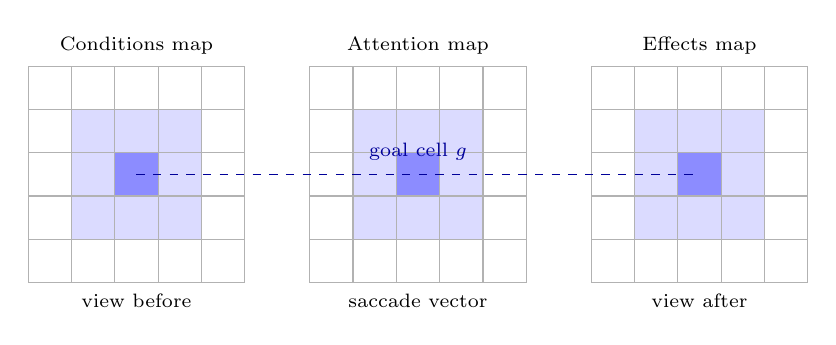
\begin{tikzpicture}[x=0.55cm,y=0.55cm]
\foreach \off/\lab/\sub in {0/{Conditions map}/{view before}, 6.5/{Attention map}/{saccade vector}, 13/{Effects map}/{view after}} {
  \foreach \di/\dj in {-1/-1,-1/0,-1/1,0/-1,0/1,1/-1,1/0,1/1}
    \fill[blue!14] (\off+2+\di,2+\dj) rectangle ++(1,1);
  \fill[blue!45] (\off+2,2) rectangle ++(1,1);
  \foreach \i in {0,...,4} \foreach \j in {0,...,4}
    \draw[gray!60] (\off+\i,\j) rectangle ++(1,1);
  \node[above,font=\scriptsize] at (\off+2.5,5.05) {\lab};
  \node[below,font=\scriptsize] at (\off+2.5,-0.05) {\sub};
}
\draw[dashed,blue!60!black] (2.5,2.5)--(9,2.5)--(15.5,2.5);
\node[font=\scriptsize,blue!60!black,above] at (9,2.6) {goal cell $g$};
\end{tikzpicture}
\caption{Three maps share one $5\times5$ lattice (the model uses $10\times10$).
The attention map is a map of retinal vectors; the sensory maps inherit order from
it through the common anchor.}
\end{figure}

\paragraph{What the sweeps show.} Numbers are from \code{docs/report.tex} (three
seeds unless noted). The maps are well ordered in prototype space: with
\code{anchor_std} 4 and neighbourhood baseline 0.5 the visual-conditions map has
Spearman 0.89, competence 0.778 and attention-map topographic error 0.07 (base:
0.78, 0.772, 0.39); with five seeds the differences among baselines are within the
seed spread. The failures found were failures of the pairing between address and
effect, not of the lattice. After each decision the attention mask resets to a
nearly flat distribution (standard deviation about 54 px on an 80 px retina), the
next step saccades to the global salience maximum, and 0.426 of goal saccades are
undone (0.331 with goal inhibition); the recorded effect is not then the effect of
the addressed saccade. \code{hold_fixation} removes the reversals (0.000) but raises
the share of test pairs with a common goal from about 0.17 to 0.68 and lowers
purity from about 0.93 to 0.84--0.86, because every scanpath starts from one hub
goal; \code{orienting_saccade} restores diversity (distinct first goals 10--13
against 1--4; pairs sharing 0.11 without inhibition) at test time only.

These results fit the claim that what has to be right is the pairing of address and
effect, not a position code. They do not test stability across starting positions;
the stable-perception test (\code{docs/draft.tex}, l.111) is still only proposed.

\section{A black-box probe of the project's maps}
\label{sec:probe}

The maps are organised over global shapes by construction: the loss uses the whole
$16\times16\times3$ fovea vector and the anchor, which is a lattice cell, and no
position label or coordinate enters it. That the maps are not retinotopic by design
is therefore not something to test. The question is whether a researcher who treats
the maps as a black box and applies a spot-probe, RF-centre protocol finds
retinotopy anyway.

\paragraph{Protocol.} The test of Section~\ref{sec:test}, implemented in
\code{scripts/probe_retinotopy.py} and \code{scripts/indirect_retinotopy_test.py}.
Each map is probed with 2000 spots of width 3 pixels at random positions in the
$16\times16$ fovea, with amplitude set to the 99th percentile of the map's weights;
readout is soft; $z$ uses 100 permutations of RF centres; the control uses 100
shuffled pixel layouts.

\paragraph{Maps.} The visual-conditions and visual-effects maps of five trained runs
at the reference configuration (\code{anchor_std} 4, baseline 0.5;
\code{tests/scanpath_eval_2026-09-27}), and two reference sets of eight batch SOMs
each (3000 images, 30 epochs): \emph{position only}, a rectangle of fixed size and
colour at random positions, which is retinotopic by design, and \emph{global shapes},
rectangles varying in size, aspect, colour and brightness (and position).

\paragraph{Rules.} Written after a first run, so post hoc. R1: every project map
shows significant retinotopy by the spot-probe protocol ($z>3$). R2: the order is
spatial beyond prototype topography ($p<0.05$ against shuffled layouts). R3: RF
centres span at most half the fovea.

\begin{table}[h]
\centering\footnotesize
\setlength{\tabcolsep}{4pt}
\begin{tabular}{@{}lccccc@{}}
\toprule
Map & $\rho$ & $z$ & gain & $p$ & RF range \\
\midrule
Position only (mean of 8)  & 0.67 & 28.2 & 0.38 & $<0.05$ in 8/8 & 0.16 \\
Global shapes (mean of 8)  & 0.47 & 11.4 & 0.05 & $<0.05$ in 1/8 & 0.38 \\
\midrule
Run 039973, conditions & 0.72 & 30.2 & 0.18 & 0.040 & 0.21 \\
Run 039973, effects    & 0.68 & 25.6 & 0.17 & 0.079 & 0.21 \\
Run 090902, conditions & 0.84 & 35.4 & 0.24 & 0.010 & 0.21 \\
Run 090902, effects    & 0.73 & 30.3 & 0.22 & 0.030 & 0.18 \\
Run 093581, conditions & 0.83 & 34.8 & 0.24 & 0.010 & 0.24 \\
Run 093581, effects    & 0.82 & 40.7 & 0.27 & 0.010 & 0.16 \\
Run 027182, conditions & 0.76 & 35.3 & 0.18 & 0.020 & 0.18 \\
Run 027182, effects    & 0.77 & 37.4 & 0.20 & 0.020 & 0.14 \\
Run 031415, conditions & 0.78 & 32.9 & 0.18 & 0.040 & 0.18 \\
Run 031415, effects    & 0.70 & 29.6 & 0.14 & 0.050 & 0.16 \\
\bottomrule
\end{tabular}
\caption{Spot probe, soft readout, width 3 px. Gain and $p$ are against shuffled
pixel layouts. Runs 039973, 090902 and 093581 are from round 4 and runs 027182 and
031415 from round 6. The last $p$ is 0.0495.}
\label{tab:probe}
\end{table}

\begin{figure}[h]
\centering
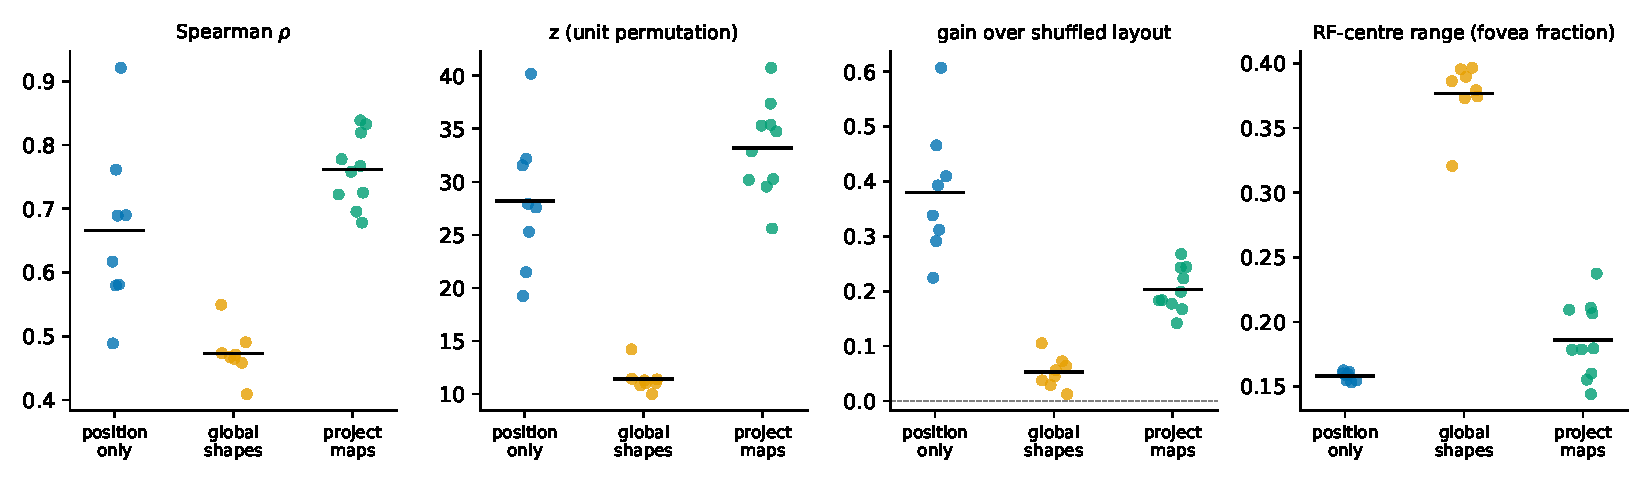
\includegraphics[width=\textwidth]{retinotopy_probe_stats.pdf}
\caption{Black-box statistics (Table~\ref{tab:glossary}) for the position-only
reference (8 SOMs), the global-shapes reference (8 SOMs) and the project's 10 visual
maps; each dot is one map and the bar is the mean. The gain panel shows the order
that depends on the spatial arrangement of the spot; the dashed line is 0.}
\label{fig:probe-stats}
\end{figure}

\begin{figure}[h]
\centering
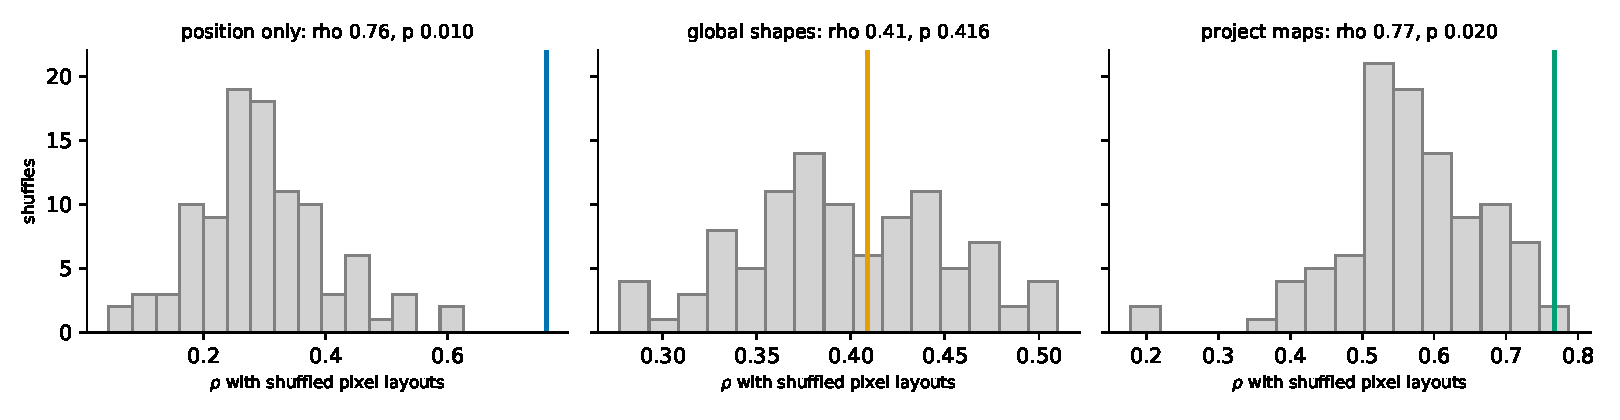
\includegraphics[width=\textwidth]{retinotopy_probe_null.pdf}
\caption{The control (steps 6--7 of Figure~\ref{fig:pipeline}). The grey bars are
the distribution of $\rho_{\mathrm{shuf}}$ under 100 shuffled pixel layouts; the
vertical line is the observed $\rho$. Position only: $\rho$ far above the shuffles.
Global shapes: $\rho$ inside the shuffles (all prototype topography). Project map
(the median by gain): $\rho$ above almost all shuffles. One map of each kind.}
\label{fig:probe-null}
\end{figure}

\begin{figure}[h]
\centering
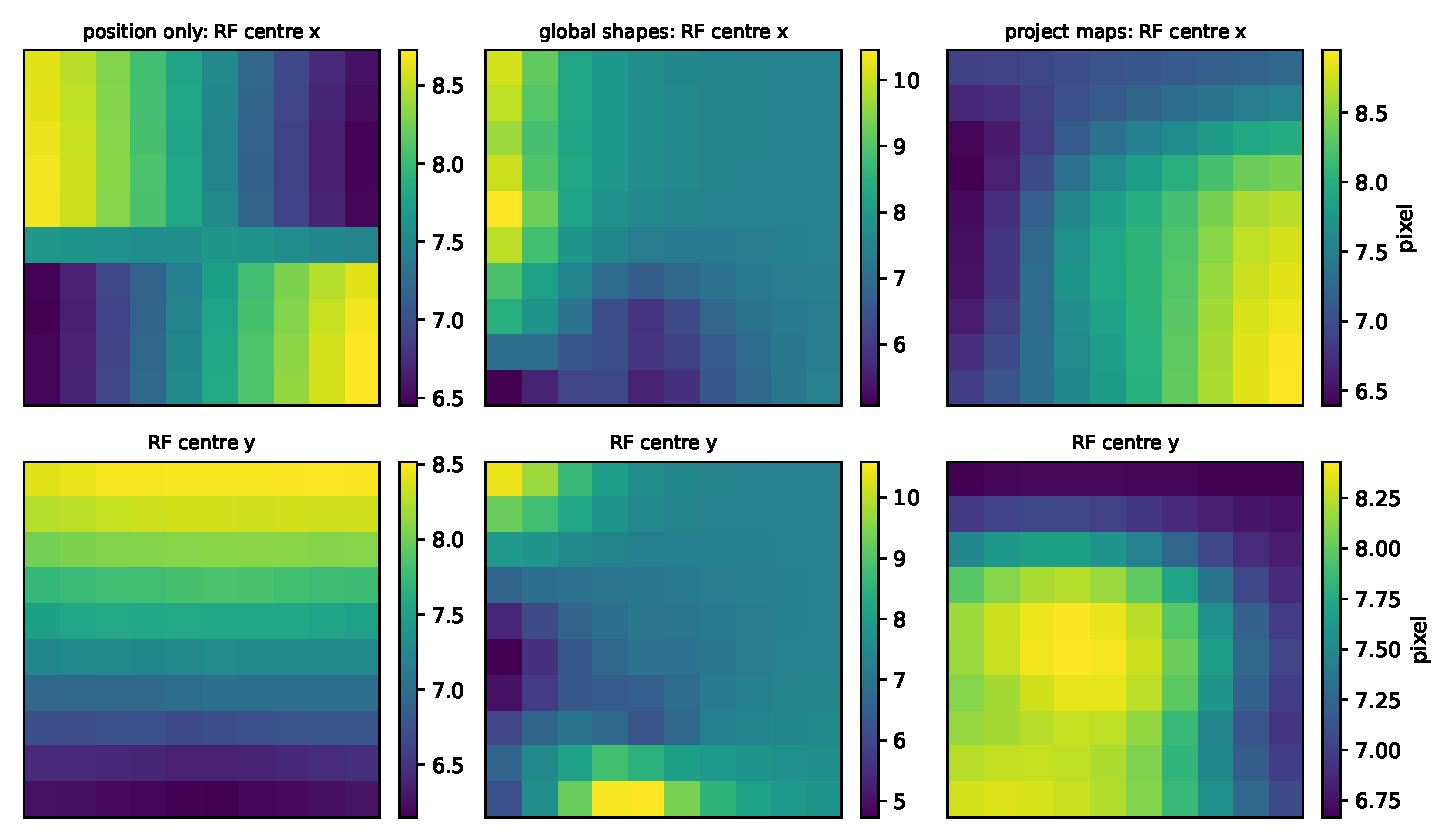
\includegraphics[width=\textwidth]{retinotopy_probe_maps.pdf}
\caption{What ordered RF centres look like (step 3). Each panel is the $10\times10$
grid; the colour of a cell is the horizontal (top) or vertical (bottom) RF centre of
that unit in fovea pixels, with its own scale. A retinotopic map shows a smooth
gradient across the grid. The position-only map has clean gradients; the
global-shapes map is patchy; the project map (the same one as in
Figure~\ref{fig:probe-null}) has gradients over part of the grid. All three cover
only a few pixels (soft readout compresses RF centres towards the mean).}
\label{fig:probe-maps}
\end{figure}

\paragraph{Result, in words.} R1 holds for 10 of 10 maps and R3 for 10 of 10. R2
holds for 9 of 10: nine maps have $p<0.05$ and the tenth has $p=0.079$. The
spot-probe protocol therefore finds retinotopy in maps trained only on global
differences among foveal images: $\rho$ of 0.68--0.84 and $z$ of 26--41, at least as
high as the retinotopic-by-design reference ($\rho$ 0.67, $z$ 28). Their gain is
0.14--0.27, which means that about 0.14 to 0.27 of correlation depends on the
spatial arrangement of the spot beyond what shuffled layouts give.

\paragraph{What the control adds.} The global-shapes reference also passes the
spot-probe test ($z\approx11$) although its gain over the control is only 0.05
(Figure~\ref{fig:probe-null}, middle): its apparent retinotopy is almost entirely
prototype-space topography. The spot-probe protocol cannot tell the two cases apart; the
shuffled-layout control can. The project maps lie in between (gain 0.14--0.27, against
0.38 for position only).

\paragraph{What it does not show.}
\begin{itemize}[nosep]
  \item The project maps score higher than the global-shapes reference. A likely reason
    is that foveal views differ mainly in where the object's features fall, so
    ``content'' and position are not separable in these data. This is untested.
  \item RF range is not diagnostic. Soft readout compresses RF centres toward the
    mean, and the position-only reference gets 0.16 against 0.38 for global shapes.
    R3 therefore passes trivially, and the earlier reading of a small range as a sign
    of local retinotopy is withdrawn.
  \item There are five distinct runs of one configuration, one spot width, one
    amplitude choice and two simple reference data sets, and the permutation $p$ has
    a resolution of $1/101$. The probe spots lie outside the training distribution.
\end{itemize}

\subsection*{Twenty runs of the champion configuration}
\label{sec:champion}

\paragraph{Expectation.} The maps are trained on view content, never on retinotopic
differences, so any retinotopy found by the black-box probe is indirect by
construction. The question here is only whether it is found. Rule fixed before the
runs (\code{predictive_remapping.md}, step 1.5): retinotopy is found in a map if the
spot-probe $z$ exceeds 3, and Phase~1 is supported if this holds in every map of the
champion configuration. Untrained maps are a pre-training reference (probe $\rho$
about 0.02, $z$ not above 3 in earlier measurements), not a classified control. The
gain $p$ against shuffled layouts is reported but not part of the rule, because it is
noisy at 100 shuffles and failed in three of the five earlier runs.

\paragraph{Maps.} The champion configuration (\code{champion.md}): reference
parameters (\code{anchor_std} 4, baseline 0.5) with goal inhibition,
\code{hold_fixation} and \code{orienting_saccade} on in training. Twenty runs of 1000
epochs: the five of Table~\ref{tab:probe} and fifteen new seeds
(\code{tests/champion_seeds_2026-10-08}), 40 maps. The probe is that of the previous
subsection with a fixed probe seed, so the values of the five older runs differ
slightly from Table~\ref{tab:probe}. The phase-encoded probe
(\code{scripts/probe_phase_encoded.py}) is a second, independent mapping: a bar
sweeps the fovea horizontally and vertically and a ring expands from the centre, and
each unit's preferred position is the Fourier phase of its response at the sweep
frequency.

\begin{table}[h]
\centering\footnotesize
\setlength{\tabcolsep}{4pt}
\begin{tabular}{@{}lcccccc|cc@{}}
\toprule
 & \multicolumn{3}{c}{Conditions} & \multicolumn{3}{c|}{Effects} & \multicolumn{2}{c}{Phase $\rho$} \\
Seed & $\rho$ & $z$ & $p$ & $\rho$ & $z$ & $p$ & cond. & eff. \\
\midrule
014142 & 0.75 & 35.9 & 0.01 & 0.82 & 47.4 & 0.02 & 0.49 & 0.60 \\
017320 & 0.82 & 46.8 & 0.02 & 0.74 & 32.3 & 0.05 & 0.61 & 0.64 \\
022360 & 0.82 & 39.9 & 0.03 & 0.66 & 30.3 & 0.02 & 0.56 & 0.42 \\
026457 & 0.83 & 49.1 & 0.01 & 0.75 & 41.5 & 0.02 & 0.55 & 0.61 \\
028284 & 0.63 & 27.2 & 0.16 & 0.79 & 40.7 & 0.02 & 0.45 & 0.61 \\
031622 & 0.86 & 51.2 & 0.01 & 0.77 & 42.1 & 0.03 & 0.62 & 0.59 \\
034641 & 0.83 & 51.9 & 0.01 & 0.75 & 37.6 & 0.06 & 0.55 & 0.48 \\
036055 & 0.83 & 55.0 & 0.01 & 0.75 & 40.1 & 0.01 & 0.57 & 0.61 \\
038729 & 0.87 & 57.2 & 0.01 & 0.76 & 43.1 & 0.05 & 0.54 & 0.58 \\
041231 & 0.82 & 44.9 & 0.02 & 0.78 & 38.0 & 0.02 & 0.54 & 0.54 \\
043588 & 0.84 & 45.0 & 0.02 & 0.76 & 43.6 & 0.03 & 0.55 & 0.54 \\
045825 & 0.85 & 48.5 & 0.01 & 0.78 & 40.9 & 0.03 & 0.57 & 0.58 \\
047958 & 0.59 & 20.5 & 0.19 & 0.65 & 26.5 & 0.19 & 0.33 & 0.42 \\
050000 & 0.57 & 21.3 & 0.22 & 0.88 & 42.7 & 0.01 & 0.22 & 0.66 \\
051961 & 0.81 & 37.6 & 0.01 & 0.77 & 39.9 & 0.01 & 0.54 & 0.56 \\
039973 & 0.55 & 21.5 & 0.11 & 0.61 & 25.3 & 0.08 & 0.42 & 0.40 \\
090902 & 0.85 & 47.6 & 0.02 & 0.79 & 40.3 & 0.05 & 0.51 & 0.62 \\
093581 & 0.84 & 47.4 & 0.01 & 0.75 & 34.2 & 0.02 & 0.58 & 0.50 \\
027182 & 0.82 & 51.4 & 0.01 & 0.74 & 38.6 & 0.01 & 0.51 & 0.59 \\
031415 & 0.62 & 25.3 & 0.13 & 0.85 & 43.3 & 0.01 & 0.43 & 0.67 \\
\bottomrule
\end{tabular}
\caption{Spot probe (soft, width 3 px; $p$ against 100 shuffled layouts) and
phase-encoded $\rho$ for the 20 champion runs. The last five rows are the earlier
runs (039973, 090902, 093581, 027182, 031415).}
\label{tab:champion}
\end{table}

\paragraph{Result.} The spot probe gives $z>3$ in 40 of 40 maps, so the rule is met.
Conditions maps: median $\rho$ 0.82 (interquartile 0.72--0.84, minimum 0.55), median
$z$ 45.9 (minimum 20.5). Effects maps: median $\rho$ 0.76 (0.75--0.79, minimum 0.61),
median $z$ 40.2 (minimum 25.3). Averaged over the two maps, run $\rho$ has mean 0.764
and standard deviation 0.065 over the 20 runs. The phase-encoded probe agrees: $z>3$
in 40 of 40 maps (median $z$ 29.1 conditions, 23.2 effects), median $\rho$ 0.54 and
0.58 (minimum 0.22). Phase-encoded and spot $\rho$ rank maps similarly (Spearman
0.52 across the 40 maps) and the phase-encoded values are lower. With no failure in
20 runs, the 95\% upper bound on the failure rate is about 14\%.

\paragraph{Reading.} This is what the argument predicts: maps organised by global view
content nevertheless read as retinotopic to an observer who treats them as a black box,
in every run and with a margin (minimum $z$ 20 against the threshold of 3). It is not
evidence of how the order arises; the probe cannot separate position from content in
these views, and that source is not under test here. Two caveats limit the strength of
the claim. First, the shuffled-layout control is passed by 32 of 40 maps ($p<0.05$);
the eight that fail are the low-$\rho$ maps (seeds 028284 and 031415 conditions,
047958 both, 050000 conditions, 039973 both, and 034641 effects at $p=0.06$), so
in those the spot order is closer to prototype topography than to spatial order, as for
the global-shapes reference. Second, the champion was chosen on five seeds (variance
analysis in \code{champion.md}), so differences among configurations are not claimed,
and run-to-run spread is large: conditions $\rho$ ranges from 0.55 to 0.87.

\section{What follows for stability}
\label{sec:stability}

If spatial order can be indirect, the positive proposal is simple. Stability is
the persistence of the neighbourhood relation between three states held on one
lattice: the view before a saccade, the saccade, and the view after it. A state is
represented by the lattice cell of its winning unit, and the relation that matters
is lattice distance, not retinal or world distance. With $g$ the goal cell and
$d_m$ the lattice distance between $g$ and the winner of map $m$ for the saccade's
attention centre and post-saccadic view, the model's match is
\begin{equation}
  \mu = \tfrac12\sum_{m\in\{\mathrm{att},\,\mathrm{eff}\}}
        \exp\!\bigl(-(d_m/\sigma_\mu)^2\bigr),
\end{equation}
with $\sigma_\mu$ the \code{match_std} parameter. The maps are trained with the
supervised topological map (STM) loss
\begin{equation}
  L=\tfrac12\sum_j d_j^2\,\phi_j\,\psi_j,\qquad
  \phi_j=e^{-\|j-r\|^2/2\sigma_r^2},\quad
  \psi_j=e^{-\|j-t\|^2/2\sigma_t^2},
\end{equation}
where $d_j^2=\|x-w_j\|^2$, $r$ is the map's own winner and $t$ the anchor. With
$\sigma_t\to\infty$ it reduces to the SOM. A position between sampled cells is
read by a Gaussian blend of prototypes, $\hat{x}(z)=W^{\top}r(z)$, so the map is a
grid-backed neural field (Amari, 1977; Erlhagen and Sch\"oner, 2002) and
interpolates between sampled states
(\code{knowledgebase/review_topographic_interpolation.md}). Learning is offline:
for each recorded saccade above threshold, the fovea two steps before is the
condition, the fovea two steps after is the effect, and the attention centre is the
action (\code{offline_controller.py}, \code{update}, l.369). The maps therefore
store condition--action--effect triples ordered on a lattice, not a function from
image to image.

\paragraph{The anchor and the limits of the claim.} The anchor resembles an
efference signal: it is written by the selected action and aligns the sensory maps
to it. We accept the resemblance. The claim is narrower than ``no CD'': the anchor
is an address on a shared lattice, it carries no forward model of the image or of
space, and the model never computes where anything will land. Anticipation
in the draft's sense is a lookup of the effect prototype at the goal cell. Three
points should be stated openly.
\begin{enumerate}[nosep]
  \item \textbf{Action coupling is required.} In the formalisation note a yoked
    agent that receives the same stream can reach high alignment on energy, but the
    anchor is then not causal. Grounding depends on acting.
  \item \textbf{Retinotopic and global leftovers.} The action space is
    retina-normalised, the attention mask is a retina-centred Gaussian, and a global
    competence modulates learning for all samples (\code{offline_controller.py},
    \code{set_hyperparams}, l.186). The reservoir in
    \code{recurrent_generative_model.py} is the only forward model and is not part
    of the main loop.
  \item \textbf{Draft framing.} The abstract of \code{docs/draft.tex} (l.64) adopts
    ``a retinotopic updating perspective''. The present view would change that
    sentence.
\end{enumerate}

\paragraph{Conclusion of the argument.} Retinotopy can be indirect, inherited from
retinal input and from alignment with the motor map. Observing it in a map, or in
the responses of a map's units around a saccade, therefore does not show that a
coordinate system is updated.

\section{Predictions that separate the views}

\begin{enumerate}[nosep]
  \item \textbf{Feature statistics shape the map.} Changing the content statistics
    of training (shape, size, view) should change the layout of a map, which is not
    expected if position is the organising axis.
  \item \textbf{Retinotopy weakens with feature dominance.} The strength of spatial
    order should fall as input becomes pooled and feature-dominated, giving a
    gradient from V1 to parietal and frontal areas.
  \item \textbf{Remapping-like responses follow lattice neighbourhood.} In the
    model: does a conditions-map unit respond to stimuli at the location its effects-map
    counterpart represents? In cortex: does presaccadic responsiveness at a unit's
    future field depend on its neighbourhood in a feature map?
  \item \textbf{Neighbourhood lesions smear goals.} Perturbing a map's neighbourhood
    should shift a saccade's goal to adjacent cells, not displace it to a wrong
    coordinate.
  \item \textbf{Coupling matters for alignment.} Disrupting action--effect
    coupling during development should degrade alignment without changing
    single-map retinotopy.
  \item \textbf{The probe result should hold under variation.} Repeat the probe of
    Section~\ref{sec:probe} with more runs, other spot widths, and maps retrained with
    different foveal content statistics; the order should follow the content
    statistics.
\end{enumerate}

\section{Objections}

\begin{itemize}[nosep]
  \item \textbf{Frontoparietal maps are retinotopic} (Mackey et al., 2017). The
    view accepts local retinotopy there. The test is whether their organisation is
    better explained by feature space plus continuity than by a coordinate frame. A
    retinotopist can describe such a map as weakly retinotopic, so the difference
    has to be mechanistic: whether stability requires a coordinate update.
  \item \textbf{Underdetermination is not support.} Showing that spatial order does not
    decide between views removes an inference; it needs the predictions above to
    support the alternative.
  \item \textbf{Wiring-cost by-product.} Topography may arise from minimising wiring
    and do no computational work; the interpolation note records this debate.
  \item \textbf{Evidence is simulated and modest.} The probe covers five runs of one
    configuration and one spot width; part of the apparent retinotopy is prototype
    topography (gain 0.05 in the global-shapes reference); the reference data sets
    are simple.
  \item \textbf{Predictive attention and fast spatiotopic effects.} Pre-saccadic
    attention shifts (Rolfs et al., 2011) and spatiotopic updating within 150~ms
    (Fabius et al., 2019) have to be explained as consequences of aligned maps. This
    is not shown here.
  \item \textbf{Discrete modules.} Grid-cell modules argue against blanket
    continuity (\code{knowledgebase/topographic_gating.pdf}, Section~5.2.2).
\end{itemize}

\section{Positioning}

\begin{table}[h]
\centering\footnotesize
\setlength{\tabcolsep}{3pt}
\begin{tabular}{@{}>{\ra}p{1.9cm}>{\ra}p{2.3cm}>{\ra}p{1.2cm}>{\ra}p{2.0cm}>{\ra}p{2.0cm}>{\ra}p{2.1cm}>{\ra}p{2.4cm}@{}}
\toprule
Account & Carried across a saccade & Global frame & Predictive model & Role of CD & Reads spatial order as & Main weakness \\
\midrule
Spatiotopic & World- or head-centred position & Yes & Eye-position signal & Updates eye position & A coordinate system & Slow, unreliable eye position; few spatiotopic cells \\
CD remapping & Retinotopic activity at the new location & No & Where each item will land & Drives the shift & An updated retinotopic map & Needs a landing signal for all items \\
Attention pointers & A few tagged locations & No & For tagged items & Drives the shift & An updated map of pointers & Background unexplained \\
Sensorimotor (O'Regan--No\"e) & Mastery of contingencies & No & General contingency knowledge & Not central & A by-product of mastery & Does not explain predictive neurons \\
Topological & Neighbourhood relation between address and effect & No & None; lookup on a lattice & Anchor on a shared lattice & Indirect, inherited from input and alignment & Simulation only; leftover retinotopic assumptions; needs action coupling \\
\bottomrule
\end{tabular}
\caption{Positioning of the topological account against the others.}
\end{table}

\section*{Open items}

\begin{itemize}[nosep]
  \item Run phase-encoded (wedge and ring) or pRF-style mapping on the maps, the
    field's standard methods, and compare with the spot-probe result.
  \item Extend the probe (Prediction 6): more runs, other spot widths, retrained
    variants. A statistic that separates genuine spatial order from prototype
    topography without a control, since RF range does not.
  \item The effect of \code{exclude_fixation} on goal execution is not written up in
    \code{docs/report.tex}; its summary file (\code{exclfix_summary.csv}) should be
    checked before citing.
  \item A stability test across starting positions, and the other predictions, have not
    been run.
\end{itemize}

\section*{References}
\addcontentsline{toc}{section}{References}

\begin{itemize}[itemsep=1pt,topsep=2pt]\small
  \item Amari, S. (1977). Dynamics of pattern formation in lateral-inhibition type neural fields. Biol Cybern 27, 77--87. \doi{10.1007/BF00337259}
  \item Arcaro, M. J., and Livingstone, M. S. (2017). Retinotopic organization of scene areas in macaque inferior temporal cortex. J Neurosci 37, 7373--7389. \doi{10.1523/JNEUROSCI.0569-17.2017}
  \item Bauer, H.-U., and Pawelzik, K. R. (1992). Quantifying the neighborhood preservation of self-organizing feature maps. IEEE Trans Neural Netw 3, 570--579. \doi{10.1109/72.143371}
  \item Bridgeman, B., Hendry, D., and Stark, L. (1975). Failure to detect displacement of the visual world during saccadic eye movements. Vision Res 15, 719--722. \doi{10.1016/0042-6989(75)90290-4}
  \item Burr, D. C., and Morrone, M. C. (2011). Spatiotopic coding and remapping in humans. Phil Trans R Soc B 366, 504--515. \doi{10.1098/rstb.2010.0244}
  \item Cavanagh, P., Hunt, A. R., Afraz, A., and Rolfs, M. (2010). Visual stability based on remapping of attention pointers. Trends Cogn Sci 14, 147--153. \doi{10.1016/j.tics.2010.01.007}
  \item DeYoe, E. A., Carman, G. J., Bandettini, P., et al. (1996). Mapping striate and extrastriate visual areas in human cerebral cortex. PNAS 93, 2382--2386. \doi{10.1073/pnas.93.6.2382}
  \item Duhamel, J.-R., Colby, C. L., and Goldberg, M. E. (1992). The updating of the representation of visual space in parietal cortex by intended eye movements. Science 255, 90--92. \doi{10.1126/science.1553535}
  \item Dumoulin, S. O., and Wandell, B. A. (2008). Population receptive field estimates in human visual cortex. NeuroImage 39, 647--660. \doi{10.1016/j.neuroimage.2007.09.034}
  \item Engel, S. A., et al. (1997). Retinotopic organization in human visual cortex and the spatial precision of functional MRI. Cereb Cortex 7, 181--192. \doi{10.1093/cercor/7.2.181}
  \item Engel, S. A., Rumelhart, D. E., Wandell, B. A., et al. (1994). fMRI of human visual cortex. Nature 369, 525. \doi{10.1038/369525a0}
  \item Erlhagen, W., and Sch\"oner, G. (2002). Dynamic field theory of movement preparation. Psychol Rev 109, 545--572. \doi{10.1037/0033-295X.109.3.545}
  \item Fabius, J. H., Fracasso, A., Nijboer, T. C. W., and Van der Stigchel, S. (2019). Time course of spatiotopic updating across saccades. PNAS 116, 2027--2032. \doi{10.1073/pnas.1812210116}
  \item Hubel, D. H., and Wiesel, T. N. (1962). Receptive fields, binocular interaction and functional architecture in the cat's visual cortex. J Physiol 160, 106--154. \doi{10.1113/jphysiol.1962.sp006837}
  \item Kiviluoto, K. (1996). Topology preservation in self-organizing maps. Proc ICNN'96 1, 294--299. \doi{10.1109/ICNN.1996.548907}
  \item Mackey, W. E., Winawer, J., and Curtis, C. E. (2017). Visual field map clusters in human frontoparietal cortex. eLife 6. \doi{10.7554/eLife.22974}
  \item Morris, A. P., Kubischik, M., Hoffmann, K.-P., Krekelberg, B., and Bremmer, F. (2012). Dynamics of eye-position signals in the dorsal visual system. Curr Biol 22, 173--179. \doi{10.1016/j.cub.2011.12.032}
  \item O'Regan, J. K., and No\"e, A. (2001). A sensorimotor account of vision and visual consciousness. Behav Brain Sci 24, 939--973. \doi{10.1017/S0140525X01000115}
  \item Rolfs, M., Jonikaitis, D., Deubel, H., and Cavanagh, P. (2011). Predictive remapping of attention across eye movements. Nat Neurosci 14, 252--256. \doi{10.1038/nn.2711}
  \item Sereno, M. I., Dale, A. M., Reppas, J. B., et al. (1995). Borders of multiple visual areas in humans revealed by functional magnetic resonance imaging. Science 268, 889--893. \doi{10.1126/science.7754376}
  \item Sereno, M. I., Pitzalis, S., and Martinez, A. (2001). Mapping of contralateral space in retinotopic coordinates by a parietal cortical area in humans. Science 294, 1350--1354. \doi{10.1126/science.1063695}
  \item Silver, M. A., and Kastner, S. (2009). Topographic maps in human frontal and parietal cortex. Trends Cogn Sci 13, 488--495. \doi{10.1016/j.tics.2009.08.005}
  \item Sommer, M. A., and Wurtz, R. H. (2006). Influence of the thalamus on spatial visual processing in frontal cortex. Nature 444, 374--377. \doi{10.1038/nature05279}
  \item Swisher, J. D., Halko, M. A., Merabet, L. B., McMains, S. A., and Somers, D. C. (2007). Visual topography of human intraparietal sulcus. J Neurosci 27, 5326--5337. \doi{10.1523/JNEUROSCI.0991-07.2007}
  \item Villmann, T., Der, R., Herrmann, M., and Martinetz, T. M. (1997). Topology preservation in self-organizing feature maps: exact definition and measurement. IEEE Trans Neural Netw 8, 256--266. \doi{10.1109/72.557663}
  \item Wandell, B. A., and Winawer, J. (2015). Computational neuroimaging and population receptive fields. Trends Cogn Sci 19, 349--357. \doi{10.1016/j.tics.2015.03.009}
  \item Xu, B. Y., Karachi, C., and Goldberg, M. E. (2012). The postsaccadic unreliability of gain fields renders it unlikely that the motor system can use them to calculate target position in space. Neuron 76, 1201--1209. \doi{10.1016/j.neuron.2012.10.034}
\end{itemize}

\end{document}
